\documentclass[11pt]{article}
\usepackage[utf8]{inputenc}
\usepackage[danish]{babel}
\usepackage{graphicx}
\usepackage{xcolor}
\usepackage{color}
\usepackage{setspace}
\usepackage{hyperref}
\usepackage{float}
\usepackage{listings}
\usepackage{lipsum}
\usepackage{dirtree}
\usepackage{url}
\usepackage[export]{adjustbox}
\usepackage{fancyhdr}
\usepackage{amsmath}
\usepackage{pdfpages}
\usepackage{booktabs}
\usepackage{listingsutf8}
\usepackage{enumitem}
\usepackage[left=1.5in, right=1.5in, top=2in, top=1in]{geometry}
%\usepackage[a4paper, top = 1in, bottom = 1in, left=1.5in,right=1.5in]{geometry}
%\usepackage[backend=biber, citestyle=ieee]{biblatex}
\usepackage{appendix}
\usepackage{comment}
\usepackage{wrapfig}
\usepackage{tikz}
\usepackage{tikz-qtree}
\usepackage{tikz-uml}
\usepackage{longtable}
\usepackage{makecell}
\usepackage{multicol}
\tikzset{baseline,every tree node/.style={align=center,anchor=north}}


\title{2. semesterprojekt}
\author{Gruppe 4}
\date{April 2021}

%\renewcommand{\baselinestretch}{1.5}
\pagenumbering{roman}
\begin{document}
\hfuzz 10000pt
\renewcommand{\refname}{Referenceliste}
\renewcommand{\figurename}{Figur}
\renewcommand{\tablename}{Tabel}
\pagenumbering{roman} % Start roman numbering
\renewcommand{\thesection}{\Roman{section}}

\begin{titlepage}
    \vspace{1cm}
    \begin{center}
        \begin{figure}[h!]
            \centering
            
\includegraphics[scale=1]{images/SDUlogo.jpg}
            
            \label{fig:SDUlogo}
        \end{figure}
        
        %Institut og skole synligt for læser
        \textsc{\LARGE Syddansk Universitet}\\[0.3cm]
        \textsc{\Large Teknisk Fakultet}\\[0.3cm]
        \textsc{\large Mærsk Mc-Kinney Møller Instituttet}\\[1.25cm]
        
        \rule{\linewidth}{0.2mm}\\[0.35cm] %Indsat en titel
        { 
            \LARGE \bfseries Udvikling af Softwareprogrammer\\[0.35cm]
            \Large \bfseries Krediteringssoftware til TV2\\[0.35cm]
        }
        \rule{\linewidth}{0.2mm}\\[1cm]
        
        \begin{table}[!h]
            \centering
            \begin{tabular}{llcl}
            \textbf{Præsenteret af:}    & &\qquad\qquad\qquad &
            \textbf{Eksamens nr.}\\
                        Jonas Beltoft & \href{jobel20@student.sdu.dk}{\texttt{jobel20@student.sdu.dk}}  %indsæt Navn og mail her
                &   &  493537\\ %indsæt eksamens nr. her
                Hans Pedersen            & 
                \href{haped20@student.sdu.dk}{\texttt{haped20@student.sdu.dk}}  
                &   & 494042\\
                Victor Bruun            & \href{mailto:vbruu20@student.sdu.dk}{\texttt{vbruu20@student.sdu.dk}}  
                &   & 177620413\\
                Jesper Diederichsen     & \href{mailto:jedie20@student.sdu.dk}{\texttt{jedie20@student.sdu.dk}}  
                &   & 496428\\
                Casper M. Stillinge     & \href{mailto:casti19@student.sdu.dk}{\texttt{casti19@student.sdu.dk}}  
                &    & 480325 \\
                Peter Ratgen             & \href{mailto:perat17@student.sdu.dk}{\texttt{perat17@student.sdu.dk}}  
                &   & 454308  \\
                \vspace{1mm}\\ %1mm vertical space
                \textbf{Vejleder:}      & &\qquad\qquad\qquad & \\
                Henrik Lykkegaard Larsen       & 
                \href{mailto:hlla@mmmi.sdu.dk}{\texttt{hlla@mmmi.sdu.dk}}              &   & \\
            \end{tabular}
        \end{table}
        
        \vfill
        \begin{table}[h!]
            \centering
            \begin{tabular}{ll}
            \textbf{Semester:} &F21\\
            \textbf{Fagkode:} &T510043101\\
            \textbf{Gruppe:} &SE04\\
            \textbf{Aflevering:} &31.08.2021\\
            \end{tabular}
        \end{table}
        
    \end{center}
\end{titlepage}
\clearpage
\section{Titelblad}
\begin{table}[h!]
    \centering
    \begin{tabular}{ll}
        \textbf{Titel:} & Udvikling af Softwaresystemer \\
        \textbf{Institution:} & Syddansk Universitet, Det tekniske Fakultet\\
        & Mærsk Mc-Kinney Møller Instituttet\\
        & Campusvej 55, 5230 Odense M\\
        \textbf{Uddannelse:} & Software Engineering\\
        \textbf{Semester:} & 2. Semester, F21\\
        \textbf{Kursuskode:} & T510043101\\
        \textbf{Projektperiode:} & F21\\
        \textbf{Omfang:} & 10 ECTS\\
        \textbf{Vejleder:} & Henrik Lykkegaard Larsen\\
        \textbf{Projektgruppe:} & SE04\\
    \end{tabular}
\end{table}

\subsection{Bidragserklæring}
\textit{Ved at underskrive dette dokument bekræfter hvert enkelt gruppemedlem, at alle hæfter kollektivt for dokumentets indhold, samt at alle har bridraget til projektets udførelse.}

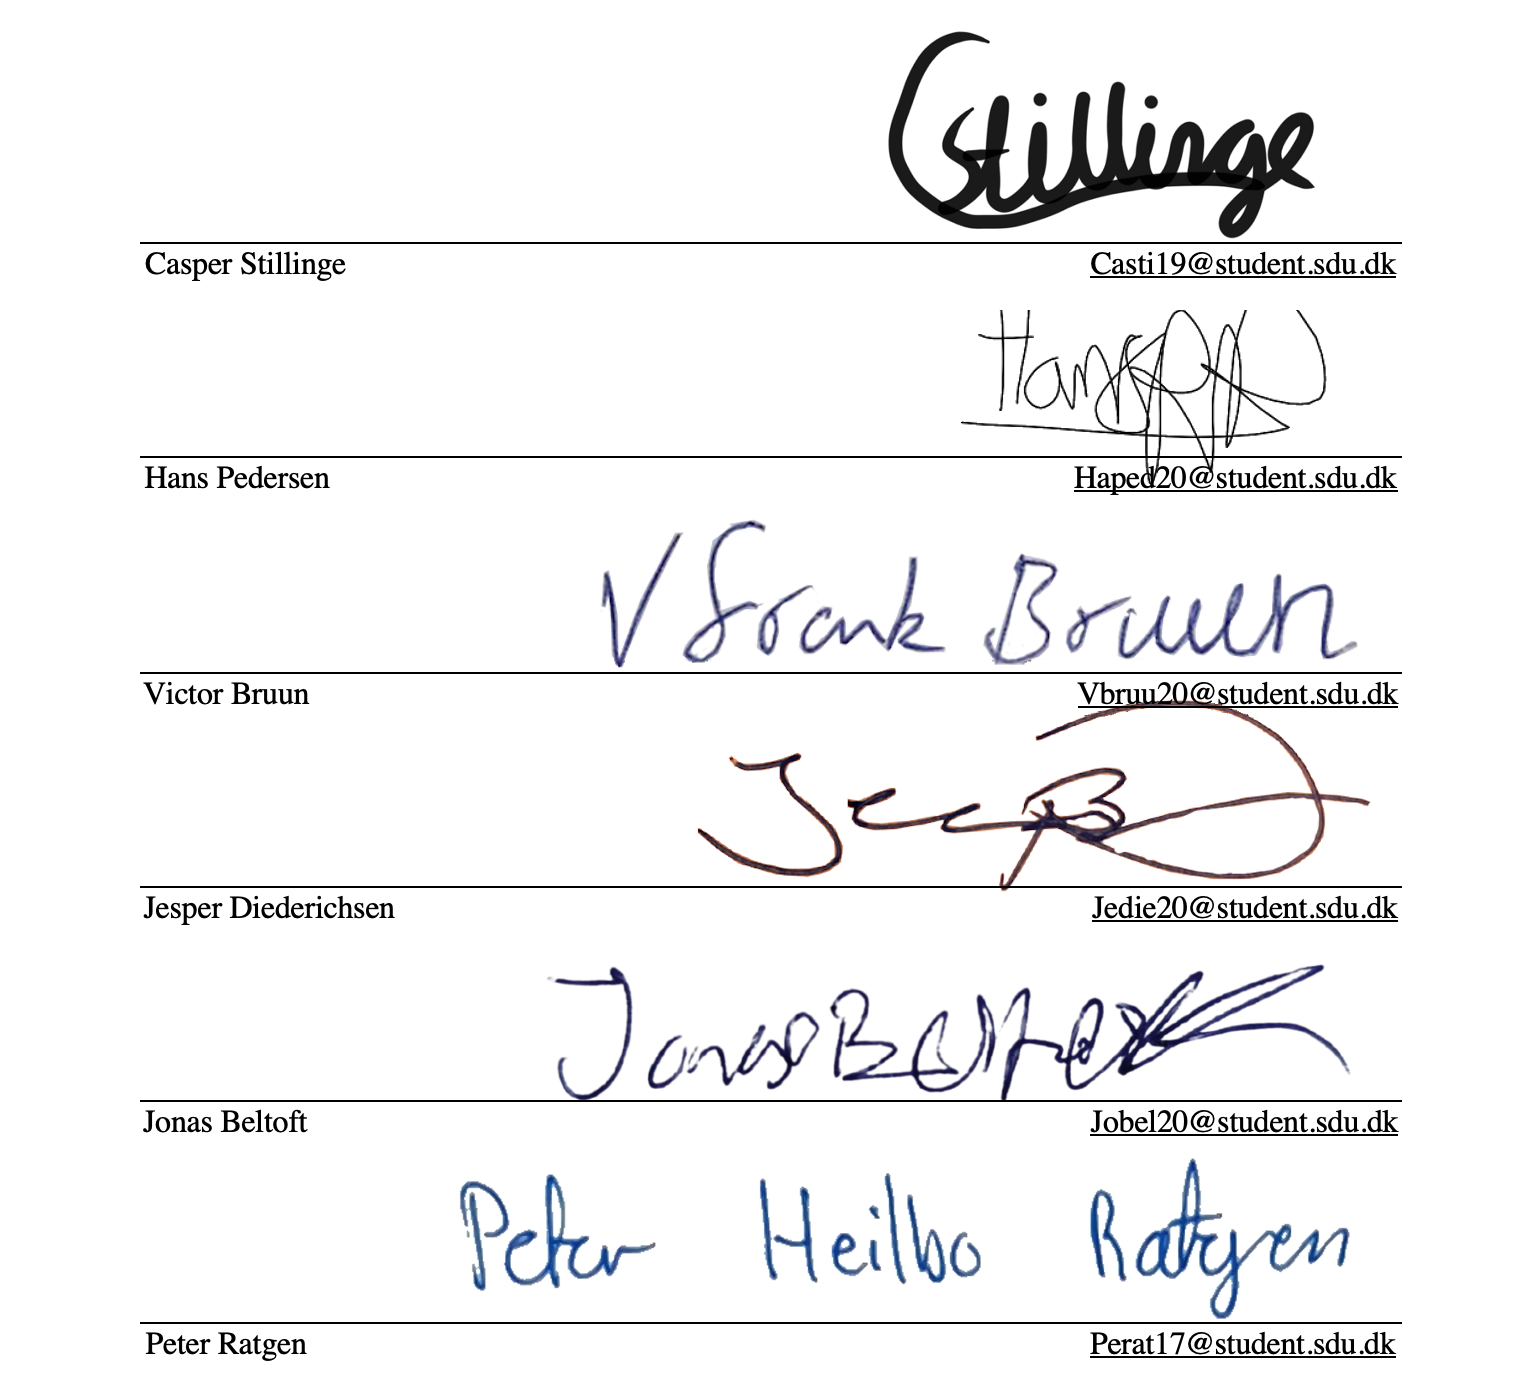
\includegraphics[scale=0.5]{images/underskrift.png}

\begin{comment}
\bgroup
    \setlength\tabcolsep{1.2cm}
     \begin{table}[h!]
     \renewcommand{\arraystretch}{1.2}
         \centering
         \begin{tabular}{lr}
             &\\&\\\hline
             Jonas Beltoft         & \href{mailto:jobel20@student.sdu.dk}{\texttt{jobel20@student.sdu.dk}}\\
             &\\&\\\hline
             Hans Pedersen        & \href{mailto:haped20@student.sdu.dk}{\texttt{haped20@student.sdu.dk}}\\
             &\\&\\\hline
             Victor Bruun        & \href{mailto:vbruu20@student.sdu.dk}{\texttt{vbruu20@student.sdu.dk}}\\
             &\\&\\\hline
             Jesper Diederichsen & \href{mailto:jedie20@student.sdu.dk}{\texttt{jedie20@student.sdu.dk}}\\
             &\\&\\\hline
             Casper M. Stillinge   & \href{mailto:casti19@student.sdu.dk}{\texttt{casti19@student.sdu.dk}}\\
             &\\&\\\hline
             Peter Ratgen         & \href{mailto:perat17@student.sdu.dk}{\texttt{perat17@student.sdu.dk}}\\
         \end{tabular}
     \end{table}
\egroup
\end{comment}

\clearpage
\section{Resumé}

\clearpage
\section{Forord}
%Hensigten med rapporten
Denne rapport er udarbejdet af gruppe SE04 på software engineering's bachelor studie gennem andet semester. Rapporten er skrevet med henblik på at oplyse læseren om, hvordan semesterprojektet er blevet udarbejdet, såvel som at vise hvordan det endelige slutprodukt fremstår. I denne rapport lægges der vægt på, at beskrive gruppens fremgangsmåde, tankeproces og arbejdsprocesser, for at kunne give et komplet billede af resultatet og vejen dertil. Gruppens arbejde med at programmere et krediteringssystem til TV 2, som skal kunne erstatte de rulletekster, der normalt ville være efter endt program, har til formål, at kunne frigive mere tid mellem udsendelserne, som TV 2 i stedet vil kunne bruge på ekstra programmer eller reklamer.\\\\
%Baggrund
Dette semesters projekt omhandler brugen af databaser og optimeret objektorienteret programmering. Projektet er i forbindelse med vores to fag også bygget op omkring en udleveret case fra TV2. I denne case findes der en beskrivelse af hvilket system der skal udvikles, hvortil der er en række krav for, hvad systemet skal kunne. Løsningen af dette projekt er yderligere udvidet med flere implementeringskrav, som vi i gruppen vurderede nødvendige, for at slutproduktet er kategoriseret som færdig og optimalt.\\\\
%Målgruppe
Vores rapport er henvendt til enhver læser, som har en interesse inden for udvikling af et softwaresystem, samt processen som ligger bag udviklingen. Rapporten henvender sig også til de medarbejdere fra TV 2 som har med vores case at gøre, for at give dem et indblik i udarbejdelsen af et softwaresystem, som kan erstatte de traditionelle rullestekster.



%Indholdsfortegnelse, der kun viser section og subsection
\clearpage
\setcounter{tocdepth}{2}
\renewcommand{\contentsname}{Indholdsfortegnelse}
\tableofcontents
\clearpage

\input{sections/Læsevejledning}
\clearpage
\section{Redaktionelt}

\begin{table}[h!]
\centering
\label{tab:1}
    \begin{tabular}{|p{40mm}|p{25mm}|p{25mm}|p{25mm}|} \hline
    \multicolumn{4}{|c|}{\textbf{Ansvarsområder}} \\ \hline
        \textbf{Afsnit}        & \textbf{Ansvarlig} & \textbf{Bidrag fra} &\textbf{\raggedright Kontrolleret af}  \\\hline
        Forside                & Victor Bruun     &          &  \\ \hline
        Titleblad              & Victor Bruun     &          &  \\ \hline
        Resumé                 &                  &          &  \\ \hline
        Forord                 & Victor Bruun     &          &  \\ \hline
        Indholdsfortegnelse    & Victor Bruun     &          &  \\ \hline
        Læsevejledning         & Victor Bruun     &          &  \\ \hline
        Redaktionelt           & Jesper Bork      & Victor Bruun         &  \\ \hline
        Indledning             & Victor Bruun     &          &  \\ \hline
        Faglige vidensgrundlag & Alle             &          &  \\ \hline
        Metode og planlægning  &                  &          &  \\ \hline
        Hovedtekst             &                  &          &  \\ \hline
        Krav                   & Jesper Bork      &          &  \\ \hline
        Analyse                &                  &          &  \\ \hline
        Design                 &                  &          &  \\ \hline
        Database Design        & Jonas            &          &  \\ \hline
        Implementering         & Peter Ratgen \newline 
                                 Hans Petersen \newline
                                 Jonas Beltoft    &          &  \\ \hline
        Test                   & Peter Ratgen     &          &  \\ \hline
        Diskussion             &                  &          &  \\ \hline
        Konklusion             &                  &          &  \\ \hline
        Perspektivering        &                  &          &  \\ \hline
        Procesevaluering       &                  &          &  \\ \hline
        Referenceliste         &                  &          &  \\ \hline
        Bilag                  &                  &          &  \\ \hline
    \end{tabular}
\end{table}

\clearpage





\setcounter{section}{0}
\renewcommand{\thesection}{\arabic{section}}
\pagenumbering{arabic}



\clearpage
\section{Indledning}
%Introduktion til TV2
Dette semesters projekt tager udgangspunkt i TV2 og deres måde at håndtere krediteringer på. TV2 er en dansk tv-station, der blev grundlagt i 1988. TV2's forretning og den måde de tjener deres penge på, fungerer ved at lave kvalitetsbevidst tv til de danske stuer. TV2 gør deres tv-kanaler tilgængelige hos forskellige tv-udbydere, oveni at de viser reklamer mellem deres programmer, som skaber deres hovedsagelige indkomst.

%TV2's plads på markedet
TV2 er, ligesom alle andre tv-produktioner, en del af et stort marked, hvor tv-skærmen er deres vindue ud til forbrugeren. På sådanne et marked handler det om at få seeren til at bruge mere tid på sine egne kanaler, frem for konkurrentens. Hvis man vil holde styr på konkurrencen mellem kanalerne, vil det nemmeste nok være at kigge på, hvor mange seere der er på en given kanal, og hvor mange minutter seeren bruger på kanalen. Ud fra Kantars seereundersøgelser kan alle og enhver se seertallene på de forskellige tv-kanaler. Kantar indsamler nemlig seeretal hvert sekund, for at kunne levere de mest præcise seeretal \cite{url_kantar} , som programlæggere i tv-branchen bruger til at forbedre tv-oplevelsen for seerene, og fastlægge hvilke tider i sendefladen, der er mest værdifulde. I følgende figur, som både er tilgængelig på Kantars hjemmeside, men også i vores case fra TV2 af, kan man se hvor mange minutter TV2s kanaler bliver set i forhold til de andre tv-kanaler.
\begin{figure}[H]
    \centering
    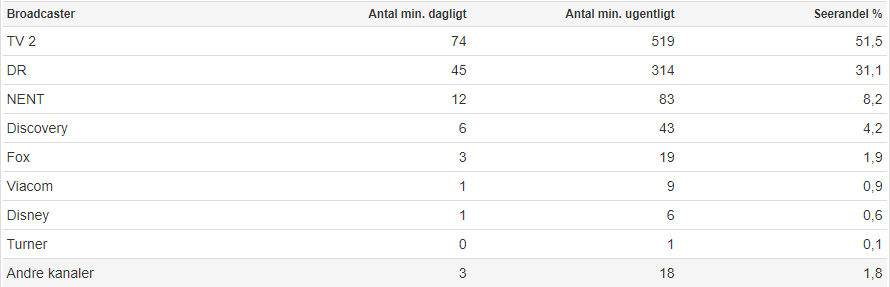
\includegraphics[width=1\textwidth]{images/Seertal.png}
    \caption{Seertid i uge 3 2020}
    \label{fig:Seertid}
\end{figure}
Det første tal der ses i figur \ref{fig:Seertid} viser, hvor mange minutter den gennemsnitlige dansker bruger på en given broadcasters tv-kanaler. Det næste tal viser hvor mange minutter det er om ugen, og det sidste tal viser, hvor stor en seerandel den givne broadcaster besidder på markedet for perioden. 
%Problemet
Som det ses har TV2 en stor seerandel, og af den grund består en vigtig del af deres indkomst af de reklamer de sender mellem deres programmer.  Men den indkomst kan blive bedre endnu, hvis de bliver bedre til at optimere tiden mellem deres programmer, vurderer TV2. Og det er netop dette problem som danner grundlag for vores case.

\subsection{Redegørelse for den udleverede case}
Når et program slutter på en af TV2s kanaler, bliver der vist rulletekster for at kreditere de medvirkende i programmet. Disse rulletekster tager dog i nogle tilfælde op til 30 sekunder, hvilket er 30 sekunder for meget. TV2 har vurderet, at hvis man kan frigøre disse 30 sekunder fra rulletekster, og bruge dem på reklamer i stedet, vil de kunne tjene op imod 60 millioner DKK om året. \cite{url_case}

Netop dette vil TV2 gøre ved at digitalisere krediteringerne, så de kan ses på nettet eller en app. For Udover at kunne sende flere reklamer mellem deres programmer, vil TV2 også have muligheden for at kreditere alle, og ikke bare de vigtigste efter endt program. I de fleste tilfælde var 30 sekunders rulletekster nemlig ikke nok til at kreditere alle medvirkende, så derfor har TV2 været nødt til at prioritere, hvilket selvfølgelig fører til at nogle krediteringer bliver glemt. Digitaliseres krediteringerne, vil alle kunne blive krediteret ligeligt, og der vil derved ikke være nogen som bliver glemt, fordi deres rolle er mindre vigtig.

Vores opgave i denne case er at skabe netop denne digitalisering af krediteringer. Det er vores opgave at udvikle et software system som kan tilføje, fjerne og redigere krediteringer i en database, hvortil vi har formuleret en problemformulering, som skal hjælpe os med at få udarbejdet en løsning på TV2s problematik med kreditering.

\subsection{Formålet med opgaven}
Formålet med det system vi har udviklet, er at gøre det lettere for producere, administratorer og TV2 som virksomhed, at kunne redigere og holde styr på krediteringer. Derudover er formålet med projektopgaven også at vi som gruppe skal forbedre vores evner inden for programmering af softwaresystemer og håndtering af databaser. Samtidigt med at vi videre udvikler vores kompetencer inden for gruppearbejde, og opsætning af et struktureret arbejdsmiljø.

Vores semesterprojekt er inddelt i to; først og fremmest har vi vores "inception", altså første halvdel. Denne del gik ud på at få udarbejdet et inceptionsdokument, som skulle lægge et fundament for vores videre arbejde med projektet. Formålet med dette inceptionsdokument var at vi som gruppe skulle ende med et veldefineret projektgrundlag, som indebar at der var styr på krav, scope og problemformuleringen. Udover dette skulle vi også klargøre, hvilke metoder vi ville benytte os af, for at kunne løse den problemformulering vi havde sat os for.

Som anden del af vores projekt, har vi den faktiske løsning af projektets problemformulering. Her har vi færdigudviklet koden, samt benyttet os af vores forarbejde i første del af projektet til at kunne besvare vores problem formulering så præcist som muligt.\\
Fordelen med at have delt vores projekt op i to halvdele, har været at vi som gruppe i første halvdel har kunne skabe os en forståelse for hvad problemet er, hvordan vi vil gribe casen an og hvordan vi som gruppe vil løse problemet på den bedst mulige måde. Dertil har vi så efterfølgende, i anden del af projektet, kunne fokusere på at følge vores planer og benytte vores forarbejde, til at udvikle det bedst mulige softwaresystem, og besvare problem formuleringen uden problemer.

\subsection{Problemanalyse}
For at gå i dybden med den stillede case fra TV2, og dermed vurdere hvad det essentielle problem er, samt skabe os en problemformulering at arbejde ud fra, har vi først analyseret casen, med fokus på at identificere, hvilke mulige problemer der er. Den case som TV2 har lavet, er relativt udpenslet, og der er ikke meget tvivl om, at det essentielle problem for dem er, at det er forbesværligt at håndtere krediteringer til produktioner på den måde, som de gør i øjeblikket, nemlig at synliggøre krediteringer i 30 sekunder efter endt program i form af rulletekster. Denne nuværende løsning er et problem, da 30 sekunder ikke er nok til at kunne vise alle medvirkende i nogle udsendelser. \cite{url_case} Der er også flere regler, som skal overholdes når der vises rulletekster, som f.eks:
\begin{itemize}
    \item Ophavsretsloven
    \item TV 2s overenskomster
    \item Kontrakter for ophavsmænd og udøvende kunstnere
    \item Almindelig god skik
\end{itemize}
Ud fra de informationer vi har erhvervet os fra casen omkring TV2s regler for hvad og hvordan der skal angives krediteringer, har vi skabt et problem træ, der skal visualisere hvordan vi ser dette problem. Dette problemtræ ses i figur \ref{fig:problemtræ}. 

Kigger man på problemtræet, vil man kunne se, at de 30 sekunder, som der maksimalt må vises rulletekster i, skaber nogle problemer for TV2. TV2 mister nemlig skærmtid, af at skulle vise rulletekster efter hvert program, men udover det, har de, som tidligere nævnt, svært ved at få plads til samtlige krediteringer på 30 sekunder. Vi vurderer derfor at årsagen, bag disse problemer er, at TV2 er begrænset til at vise krediteringer i tv'et, og dette problem kan løses ved at flytte krediteringer over på et andet medium end tv-skærmen. 

 \begin{figure}[H]
    \centering
    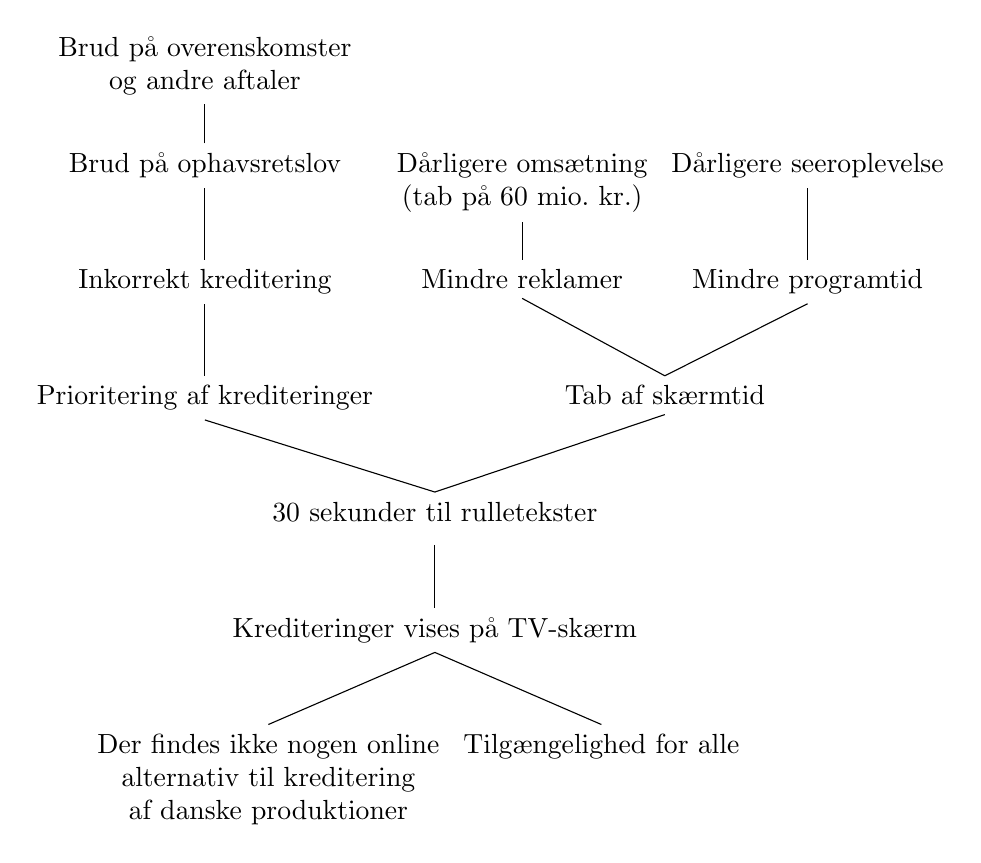
\begin{tikzpicture}[grow'=up]
        \tikzset{level distance=42pt}
        \Tree [ .{30 sekunder til rulletekster} 
                [.{Prioritering af krediteringer}
                    [.{Inkorrekt kreditering}
                        [.{Brud på ophavsretslov} 
                            [.{Brud på overenskomster\\og andre aftaler} ] ]
                    ]
                ]
                [.{Tab af skærmtid}
                    [.{Mindre reklamer} 
                        {Dårligere omsætning\\(tab på 60 mio. kr.)} 
                    ] 
                    [.{Mindre programtid} 
                        {Dårligere seeroplevelse} 
                    ] 
                ]
            ] 
        \tikzset{grow'=down}
        \Tree [ .{\\} 
                [.{Krediteringer vises på TV-skærm} 
                    [.{Tilgængelighed for alle} ]
                    [.{Der findes ikke nogen online\\alternativ til kreditering\\af danske produktioner} ]
                ]
            ]
              
    \end{tikzpicture}
    \caption{Problemtræ omkring de informationer, der er givet i casen.}
    \label{fig:problemtræ}
\end{figure}

\subsection{Problemformulering}
Ud fra vores analyse af TV2s case, er vi kommet frem til en problemformulering og dertilhørende underspørgsmål. Vores problemformulering har vi formuleret således:\\
\linebreak
\textbf{Hvordan kan vi udvikle en prototype til et krediteringssystem, der vil kunne erstatte de klassiske rulletekster efter et afsluttet program?}
\\\\
Og vores underspørgsmål, til at supplere problemformuleringen lyder således:
\begin{itemize}
    \item Hvordan er reglerne for krediteringer for danskproducerede programmer?
    \item Hvilke informationer skal og må inkluderes i krediteringer?
    \item Hvordan kan sådan et program gøres mest mulig brugervenligt(tilgængeligt) for både seer og administrator?
    \item Hvordan kan vi sikre et velstruktureret program, der mindsker fejl og ventetid samt strukturere databasen således, at der undgås fejl, duplikering af værdier og null-værdier?
\end{itemize}

\subsection{Afgrænsninger}
Projektet kan blive stort, og der er et utal af muligheder for, hvordan man kan skabe en overskuelig softwareløsnign på TV2s problem. Derfor har det også været vigtigt for os, at begrænse os. Vi vil gerne undgå at bruge for meget tid på, funktionaliteter, som ikke er vigtige, og lægge vores kræfter i de ting, som vi ved, vi kan overskue at gennemføre, og som der er tid til at få udviklet. Gruppen holder sig derfor til, udelukkende at arbejde med danske krediteringer, og undgår derved bevidst krediteringer til udenlandske shows og programmer. Gruppens produkt udarbejdes også kun som en prototype, og det betyder, at produktet ikke vil blive udviklet til et færdigt produkt, som vil opfylde alle givne krav fra TV2s side af. Krediteringerne vil dog stadig overholde de givne regler for krediteringer, men kommer til slut ikke til at være et produkt TV2 kan adaptere direkte over til. 

\section{Fagligt vidensgrundlag}
\vfuzz=100pt
\hfuzz=100pt

Vidensgrundlaget for udarbejdelsen af denne rapport gennemgås i dette afsnit, med redegørelse for relevante begreber, teori samt det faglige vidensgrundlag. Dette afsnit tager udgangspunkt i det tilsvarende afsnit fra inceptionsdokumentet med tilføjelser samt udbedringer. 
Gruppens viden og færdigheder omkring udviklingen af software programmet, samt metode og planlægning, bygger på det lærte indhold fra de øvrige fag på 2. semester. 

\subsection{Kravudvikling}

Når kravene til et system skal findes vil man som regel følge et workflow, der sikrer at kravene bliver så præcise, komplette og konsistente som muligt. 
\begin{itemize}
    \item Præcise krav, da tvetydige krav kan fortolkes på forskellige måder. 
    \item Komplette krav, så de indeholder beskrivelser af alle aspekter. 
    \item Konsistente krav der er konsekvente. Kravene må altså ikke modsige hinanden eller være i konflikt med hinanden.
\end{itemize}
Kravene til et softwaresystem er derfor vigtige at have styr på, da de fastsætter hvad systemet skal gøre, og definerer begrænsninger for dets udvikling og drift. 


For at få et optimalt workflow til at få skabt nogle gode krav, har vi i gruppen kigget på at lave en brugsmønstermodel, også kaldet use-case. 
Det indebærer, at vi først har fundet de aktører, der forbindes med systemet. For at identificere en aktør kan man spørge: "Hvem eller hvad bruger systemet?" "Til hvad?" og "Hvorfor?". Man kan kigge på hvilken rolle de spiller i interaktionen med systemet. Man kan også spørge, hvilke andre systemer bruger eller bidrager med til systemet. Når man er afklaret med hvilke aktører der er, skriver man dem op i listeformat, hvor man inkluderer aktørernes navne, deres mål (hvad og hvorfor) og deres bidrag.

Næste punkt i en brugsmønster-model er at finde og identificere brugmønstre.
Når man identificerer brugsmønstre vil man gå ud fra listen over aktører, og stille sig selv en række spørgsmål. Hvilke mål har en aktør? Det er skrevet ned i listen, og man kan derfor lave et brugsmønster til hvert mål aktøren har. Hvilke funktioner vil en specifik aktør have af systemet? Til det kan man lave et brugsmønster til en funktion, der giver målbare resultater til aktøren. Gemmer systemet information, som den henter frem? I så fald, for hvilken aktør gør den det? Dette er også værd at overveje, når der skal laves brugsmønstre. Ligeledes som med aktørerne, laves der en liste over brugsmønstre, der indeholder deres navne og deres formål.
Til slut skal der identificeres systemgrænser. Til det skal der først tegnes et brugsmønster diagram med aktører, de fundne brugmønstre, og linjer herimellem, der forbinder aktøren med de relevante brugsmønstre. Nu er det vigtigt, at man evaluerer, sine brugsmønstre, aktører og emnet. Ud fra sine evalueringer kan man nu danne sig et billede af, hvilke krav, der stilles til systemet, og man ender derfor med en skitsering af en kravspecifikation til systemet.


\subsection{Analyse af brugsmønstre}
Brugsmønstrene kan derefter analyseres og der udarbejdes sekvensdiagrammer og operationskontrakter, som kan overføres til et klassediagram og derved opbygge et overblik over systemet. 

Dette foregår ved at der bliver udvalgt en række brugsmønstre til analysen. Til hvert af disse udformes et sekvens diagram, som viser det specifikke hændelsesforløb indefor et brugsmønster og de objekter og den adfærd der er beskrevet i brugsmønsteret. 

Ud fra skevens diagrammet laves en operationskontrakt, som beskriver de forpligtigelser operationen har, samt hvilke ændringer der forekommer i systemet efter operationen er kaldt. 

Dernæst kan et systemsekvens diagram udarbejdes. Et systemsekvens diagram er et udvidet sekvensdiagram, som viser den komplette række af begivenheder der udføres når operationen udføres. Til sidst kan det udvidet sekvens diagram overføres til et klassediagram. 


\subsection{Arkitektonisk design}
Arkitekturen for systemet fastlægges tidligt i elaborationsfasen, når det er Unified Process der bliver benyttet. Det er vigtigt for ethvert software projekt at systemets arkitektur er velovervejet og godt udarbejdet, da det vil få stor betydning for det endelige produkt kvalitet. Designet fastlægges hovedsaligt ud fra de ikke-funktionelle krav, som f.eks. at vi i dette projekt har et krav om en tre-lags arkitektur, der allerede har sat bestemte rammer for det arkitektoniske design. 


\subsection{Brug af SCRUM i projektet}
SCRUM er et agilt projektudviklings værktøj der primært er udviklet til udviklingen af software. SCRUM bygger overordnet på 3 artefakter. Product backlog, sprint og inkrementer. 

\paragraph{Product backlog}
Product backlog er en liste af opgaver/krav der skal implementeres på et produkt for at nå et fælles produktmål. Emnerne i product backlog er prioriteret således at det mest nødvendige implementeres først. Disse emner er hvad der indgår i det næste SCRUM artefakt, sprintet.

\paragraph{Sprint}
Et sprint er en plan for at implementere en mængde af krav, for at opnå et mål. Man deler sprintplanlægningen op ved at besvare følgende spørgsmål om det. hvorfor, hvad og hvordan. Ved at finde ud af hvad målet for sprintet er, har man hvorfor sprintet er vigtigt. Derefter vælges de emner i product backlog, der, når implementeret, opnår dette mål. Disse emner sættes ind i et såkaldt sprint backlog der fungerer på samme måde som product backlog, blot kun for et sprint. Dette sprint backlog er også prioritet er derved har man en plan for sprintet, og derved besvaret hvordan.

\paragraph{Inkrement}
Et inkrement er et betydeligt skridt på vej hen mod det endelige produkt. Et inkrement skal præsentere en virkende del af programmet. Det vil sige der hele vejen igennem er et kørende program, der udbygges med features inkrement efter inkrement. 

SCRUM benytter sig også af nogle roller, der er essentielle for succesfuld brug af værktøjet. 

\paragraph{SCRUM master}
En SCRUM master står får at få etableret SCRUM-flowet. Dette gøres ved at der skabes en fælles forståelse for hvordan arbejdsprocessen ser ud, og hvilke værktøjer der anvendes og hvordan. Det er SCRUM masterens opgave at sørge for hele processen bliver overhold, for hvis ikke dette formås, forsvinder alle fordelene ved SCRUM. 
%I Gruppen har Hans Pedersen ageret som SCRUM master

\paragraph{Product owner}
En product owner er ansvarlig for product backlog. Det er vigtigt at de emner der skal op på product backlog, går gennem product owner, så de har det fulde overblik over hvad produktet indeholder. Derfor er der også kun én product owner, så man sikrer sig at der altid er en der har 100\% styr på hvordan produktet ser ud, og hvordan det skal se ud. Idet gruppen er lille nok til kun at indeholde et SCRUM team, har gruppen udnævnt at product master er hovedansvarlig for produktet. 
%I gruppen har Jonas Beltoft ageret som product owner, da han er iderig, og har gode evner indenfor programmering, og visualisere sig programmer.

\paragraph{Developers}
Developers, eller udviklere, er dem der sørger for at et sprint rent faktisk også arbejder fremad mod et inkrement. De står for at implementere de emner der er tilføjet til sprint backlog
%I gruppen er alle medlemmer indgået som udviklere.

\subsection{Objekt-orienteret programmering}
\paragraph{Hvad er OOP?}
Objekt-orienteret programmering (eller OOP), er et programmeringsparadigme baseret på et koncept af "objekter". Disse objekter kan indeholde en række data, generelt kaldet attributter. Kode kan være skrevet i form af en procedure, der skal lave noget bestemt, dette bliver kaldt en metode. Et eksempel kunne være at kode en person, denne person ville være et objekt. Personen har flere forskellige metoder til at kunne tale, bevæge sig, trække vejret osv. Person objektet skal også have nogle attributter så som en højde, deres køn, deres alder osv. 

Ved brug af Java-kodesprog i dette projekt kommer vi til at gøre stor brug af klasser. Når man definerer en klasse, opretter man egentlig et blueprint til et objekt. Heri defineres ikke direkte data, men der defineres hvad der skal gøres med noget data der er givet til objektet.

\subsubsection{OOP's fire basale koncepter }

    \paragraph{Indkapsling} 
    Når man snakker om indkapsling inden for OOP, så betyder det at nogle data eller noget funktionalitet bliver indkapslet. Dette gøres ved hjælp af Access modifiers. Access modifiers hjælper til at bestemme, hvem der har adgang til data og funktioner, og hvor meget der er adgang til. Der findes en række forskellige access modifiers som kan ses på tabellen \ref{tab:Access modifier} på side \pageref{tab:Access modifier}. Indkapsling er en god måde at lave dataskjulning for andre klasser. Indkapsling gør det også nemmere at teste produktets sikkerhed. 
        
        \begin{table}[H]
        \centering
            \begin{tabular}{p{2cm}|p{2cm}|p{2cm}|p{3cm}|p{2cm}}
                \textbf{Access Modifier} & \textbf{Inden for klassen} &
                \textbf{Inden for pakken} & \textbf{Uden for pakken kun af
                subklasser} & \textbf{  Uden for pakken} \\
                \hline
                Private   & X &   &   &   \\
                \hline
                Default   & X & X &   &   \\
                \hline
                Protected & X & X & X &   \\
                \hline
                Public    & X & X & X & X \\
            \end{tabular}%
            \caption{Liste over tilgange ved de forskellige access modifiers}
            \label{tab:Access modifier}
        \end{table}

    \paragraph{Abstraktion} 
    Abstraktion er en måde på at gemme specifikke værdier og metoder. Abstraktion kan ses som en udvidelse på indkapsling, siden det kan gemme information eller metoder for ekstern kode. Dette gør interfacet af objekter meget simpelt. F.eks. kan abstraktion forstås ved at kigge på kroppen, vores skind fungere som an abstraktion til at gemme hvad der foregår inde i kroppen.

    \paragraph{Nedarvning} 
    Nedarvning kommer fra at være en subklasse. Her nedarver subklassen attributter og metoder fra dens superklasse. Dette gøre det muligt at nemmere kunne genbruge kodestykker. Derudover bruges det også til metodeoverskrivning så man kan opnå runtime polymorfi. 
    Imodsætning til nedarvning, hvilket er it såkaldt "IS-A" forhold, findes der også et "HAS-A" forhold, et aggregat.
    Et HAS-A forhold beskriver de gange hvor et objekt gøre brug af et andet objekt til at gemme data. F.eks. hvis man har en kunde med nogle informationer inde i et objekt, så kan der herunder oprettes et adresse objekt hvilket indeholder information som by, kommune, post nummer osv. 
    Et aggregat kan være god at bruge i situationer hvor en stor klasses information kan deles ud i mindre bidder.  Det hjælper også meget på kode genanvendelse.
    I den virkelige verden kan vi forestille os nedarvning ved at kigge på insekter. Alle insekter har lignende egenskaber så som at have seks ben eller et exoskelet. Altså ville en grasshoppe eller myre have nedarvet disse egenskaber fra superklassen af insekter.
    \paragraph{Polymorfi} 
    Polymorfi er muligheden for at et objekt kan tage flere former. Dette gør at vi kan implementere en metode fra en superklasse i en subklasse på forskellige måder. 
    Det ville altså sige at hvilket som helst subklasse objekt i Java kan hvilken som helst form som er i superklassens hierarki, inkluderende sig selv.
    Generelt er der to typer af polymorfi:
    \begin{itemize}
        \item Dynamisk polymorfi 
        \subitem 
        Dynamisk polymorfi er også kendt som run-time polymorfi. Dette kan beskrives ved at tænke på superklasse-subklasse forhold. De begge har den samme metode, og subklassen har overskrevet superklassens metode (metode overskrivelse).
        Når et objekt bliver tildelt en klasse reference, og en metode fra objektet bliver kaldt, så er det metoden indeni objektets klasse, der bliver udført. Der bliver altså ikke kaldt metoden fra reference klassen, hvis altså referencen er en superklasse. %skal lige læses igennem, der er nogle lange sætninger
        \item Statisk polymorfi 
        \subitem Statisk polymorfi er  også kendt som compile-time polymorfi eller metode overbelastning. Dette betyder, at man har angivet flere af de samme metodenavne, men med forskellige argumenter. Det betyder altså, når man kalder sådan en metode, så ville kompilatoren beslutte hvilken metode, der bliver kørt i forhold til hvilke parametre, der er angivet.
    \end{itemize}
    
\subsection{Trelagsarkitektur}
Trelagsarkitekturen er en softwarearkitektur, der deler programmet op i tre lag.
Et præsentationslag, et logiklag og et datalag: 
\begin{itemize}
    \item Et præsentationslag som udelukkende står for at forsyne brugeren med
        en brugerflade og hente information fra brugeren og med den information
        kommunikere med det næste lag, logiklaget.
    \item Logiklaget (også kaldet domænelaget) står for alle de logiske
        operationer som er associeret med de gældende elementer i
        præsentationslaget på baggrund af den information, som brugeren har
        indtastet. Logiklaget kommunikerer også med datalaget, og kan her
        sammenholde information fra brugeren med det i databasen for at tage en
        beslutning om, hvad programmet skal gøre.
    \item Datalaget står for at lagre systemets data som logiklaget kan anvende.
\end{itemize}

Figur \ref{fig:trelagsarkitekur} beskriver denne lagdeling. 

\begin{figure}[H]
    \centering
    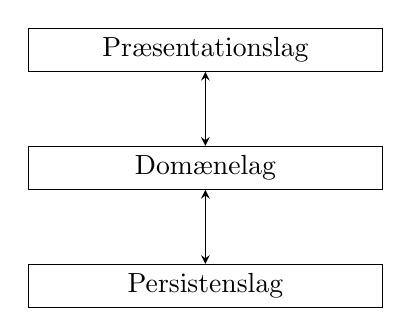
\begin{tikzpicture}
        \node[rectangle, draw, minimum width=4.5cm] (presentation) at (0,0) {Præsentationslag};
        \node[rectangle, draw, minimum width=4.5cm] (domain) at (0,-1.5) {Domænelag};
        \node[rectangle, draw, minimum width=4.5cm] (persistenslag) at (0,-3)
            {Persistenslag};
        \draw[stealth-stealth] (presentation) -- (domain);
        \draw[stealth-stealth] (persistenslag) -- (domain);
    \end{tikzpicture}
    \caption{Beskrivelse af en trelagsarkitektur}
    \label{fig:trelagsarkitekur}
\end{figure}

For en succesfuld anvendelse af trelags arkitekturen vil brugeren udelukkende
blive præsenteret for præsentationslaget og behøver ingen viden om de
underliggende lag, da al kommunikation mellem bruger og program sker i dette
lag. Brugen af trelags arkitekturen giver nogle fordele. 
\begin{itemize}
    \item Først og fremmest kan udarbejdelsen af de forskellige lag uddelegeres
        således at de udvikles samtidig. Dette gør udviklingen af programmet
        hurtigere 
    \item Da al logikken sker et sted, bliver programmet mere
        skalérbart idet at koden/programmet ikke er kludret sammen og har for
        mange indgangspunkter.  
    \item Hvis et lag bryder sammen eller ikke
        virker, påvirkes de andre ikke, da de er opdelt.
    \item Grundet at trelags arkitekturen opdeler præsentationslaget og
        datalaget med et logiklag, vil man med korrekt implementering kunne
        sikre, at en bruger ikke får tilladelse til at tilgå data, som ikke er
        tiltænkt dem. 
    \item Lagdelingen bevirker at man kan ændre på implementeringen af et givent
        lag uden at de andre bemærker det.
\end{itemize}

\subsection{Unified Process} \label{section: Unified Process}
Unified Process (UP) er en iterativ og trinvis udviklingsproces. UP er delt op i 4 trin, eller faser, disse og deres definitioner er:
\begin{itemize}
    \item Inceptionsfasen
        \subitem I inceptionsfasen skal man finde ud af projektets gennemførlighed, finde frem til vigtige krav og identificere potentielle risici.
    \item Elaborationsfasen
        \subitem I elaborationsfasen skal der laves en arkitekturprototype, oveni at risikovurderingen forbedres. Hertil skal hovedparten af brugsmønstrene findes, samt at der skal lægges en plan for konstruktionsfasens forløb.
    \item Konstruktionsfasen
        \subitem I konstruktionsfasen færdiggøres den endelige identifikation af brugsmønstre, samt disses beskrivelse og realisering. Analyse, design, implementation og test færdiggøres også i denne fase. Undervejs redigeres projektets risikovurdering.
    \item Transitionsfasen
        \subitem I denne fase rettes fejl, og brugerne forberedes på at anvende softwaren. Her laves også manualerne og anden dokumentation, til sidst gennemføres et review af projektet. 
\end{itemize}
 
En vigtig pointe omkring UP er at det er en proces drevet af brugsmønstre (use cases), samt at der fokuseres på risikostyring og arkitektur. Og som tidligere nævnt er der fokus på iterationer og en trinvis udviklingsprocess. Dette betyder at systemet udvikler sig trinvist for hver iteration.


\subsection{UML}



UML eller Unified Modeling Language, tilbyder en måde at visualisere et systems arkitekturelle blueprints i et diagram. 





\subsubsection{Klassediagrammer}

Det er bl.a. brugt til at lave Class Diagrams, da det giver en oversigt over hvilke klasser der er i et program, hvilke attributter og metoder de har, samt disses synlighed (Access Modifiers). UML anfører også sammenhængen mellem klasserne, om de fx nedarver fra klassen eller andet, hvilket er en stor del af grunden til at man bruger UML.  Ud fra det kan man aflæse hvordan forskellige klasser bliver brugt andre steder i programmet, og derved få en bedre forståelse for hvordan programmet virker, uden at man har set programmet køre. Der er særlig notation til at fremhæve alle OOP's fire basale koncepter, hvilket gør det muligt at udarbejde og/eller visualisere præcist det program, der er ønsket. Øverst ses navnet på den klasse, der beskrives. 

\begin{wrapfigure}{r}{0.30\textwidth}
    \vspace{0cm}
    \begin{tikzpicture}
        \umlclass{Kunde}{
        \small - navn: String\\
        \small - email: String\\
        \small- saldo: long\\
        \small- kurv: Vare[]\\
        }
        {
        \footnotesize+ Kunde()\\
        \footnotesize+ tilføjTilKurv(Vare) : void\\
        \footnotesize+ købVarerIKurv() : Vare[]\\
        }
        \umlclass[y=-5.5]{Vare}{
        - navn: String\\
        - pris: Double\\
        - udløbsdata: Date\\
        }{
        + Vare()\\
        }
        \umlcompo{Kunde}{Vare}
    \end{tikzpicture}
   % \centering
    %\includegraphics[width = 0.25\textwidth]{Images/UML eksempel.png}
  \caption{UML klassediagram for sammenhængen mellem en Kunde og en Vare}
  \label{fig:UML eksempel}
\end{wrapfigure} 

I sektionen under, er alle klassens attributter, og under dem er klassens metoder. Hvis klassen har en eller flere constructors, kan disse også ses, da de har det samme navn som klassen. På grund af alt dette, kan UML være et meget kraftfuldt værktøj under udviklingen af et objektorienteret program, da man kan visualisere alle de objekter og klasser, der bliver lavet og instantieret. Samt sammenhængen mellem disse objekter og klasser. UML bruges også til andre ting, såsom brugsmønster-diagrammer, som giver et overblik over aktører og de brugsmønstrer de interagerer med. Dette er en anderledes måde at modellere på, men det er alt sammen under UML, da det er en universel måde at forbinde elementer på, i en visuel kontekst.


\subsubsection{Beskrivelse af database med UML}
UML kan også bruges til at vise en database. Det ses nemt hvilken udgave, der er brugt, da man her vil se notationer så som \{PK\} som beskriver at denne attribut er en primær nøgle i denne tabel. Hver kasse er her ikke en klasse, men en tabel. Den har kun attributter, da en tabel ikke har funktioner. Et UML diagram over en database vil også have forskellige måder at visualisere sammenhæng mellem tabellerne.
Klassediagrammet som beskrevet har kun én standardiseret måde at forbinde klasserne på, hvilket gør det nemmere at lære og hurtigere at finde ud af, hvad der menes med de forskellige symboler man støder på, hvorimod et UML diagram over en database har flere forskellige måder at vise sammenhæng på, selvom de viser det samme. I klassediagrammet vil man se symboler som f.eks. betyder at denne klasse nedarver fra en anden klasse, eller bl.a. viser at den ene klasse "bruger" eller "afhænger" af en anden klasse. Dette finder man ikke i et database UML diagram. Her viser forbindelserne, hvor mange elementer, der kan være, f.eks. kan en kunde købe mange varer, men en type vare kan købes af mange forskellige kunder, så det vil kaldes en mange til mange forbindelse. Dette kan noteres på forskellige måder, f.eks. med crows foot, Chen eller andre. Vi som gruppe vil bruge Crow´s foot, som er en meget simpel måde at vise, om det er 0, 1 eller flere. Disse notationsformer er også brugt i ER og EER modeller, men det betyder ikke at et UML diagram er det samme som et ER eller EER diagram, da de ikke går direkte ned i databasen, men er mere en overordnet beskrivelse og kan vise andre ting end UML kan.

\subsection{MoSCoW}
MoSCoW er en model der bruges når en liste af krav skal prioriteres. Kravene indeles i 4 grupper, efter hvor vigtige de er for projektets succes. Her startes der med "Must Have" som er de vigtigste krav og som er nødvendige for at projekt bliver en succes. Dernæst kommer "Should Have" som er krav, der ikke er nødvendige, men det vurderes at de giver en tilstrækkelig værdi til projektet, i forhold til arbejdsindsatsen. "Could Have" er krav som ikke er vigtige for projekts gennemførsel, de kan tages med i tilfælde af overskydende arbejdsressourcer, men der planlægges ikke efter, at de skal medtages. Til sidst findes "Would Have" som er krav, der giver mening for projektet, men er valgt fra i den pågældende udgave af projektet. 

\subsection{FURPS+}

\begin{itemize}
    \setlength\itemsep{0em}
    \item Usability
    \subitem "Usability" handler om de menneskelige interaktioner med programmet. Det gælder om at se på, hvor effektivt programmet er. Er dokumentationen for programmet i orden og uddybende nok, til at forklare hvad programmet står for.
    \item Reliability
    \subitem "Reliability" omhandler det, der vedrører oppetid, præcision i systemets beregninger.
    \item Performance
    \subitem "Performance" drejer sig om, hvordan systemet skal reagere på større mængder af information.
    \item Supportability
    \subitem "Supportability" omhandler krav, som vedrører testbarhed, kompatibilitet, konfigurerbarhed.
    \item Plus
    \subitem "Plus" er den del af FURPS+ der indeholder begrænsninger og specifikke krav for systemet.
    \begin{itemize}
        \item Design constraints
        \subitem Man kigger på designmæssige begrænsninger, der kunne være for projektet. Ændrer I/O enheder eller den valgte DBMS, hvordan softwaren skal bygges?
        \item Implementation requirements
        \subitem Man kigger også på implementationen og dets krav, og beskriver, hvordan programmørene skal forholde sig. Skal de bare forholde sig til standarderne?
        \item Interface requirements
        \subitem Interface krav kigger på om, der er nogle interfaces som programmet skal fungere på eller med.
        \item Hardware requirements
        \subitem Til sidst er der hardware krav, hvor der kigges på, om der er nogle krav til hvilken hardware systemet skal interagere med eller kører på, og om det skaber nogle forudsætninger for produktionen. 
    \end{itemize}
\end{itemize}

\input{sections/3metoder_og_planlægning}
\section{Hovedtekst}
I dette afsnit dokumenteres det faktiske arbejde, samt de opnåede resultater fra både 1. og 2. iteration.

\subsection{Overordnet krav}
De overordnede krav er udformet på baggrund af den stillede case fra TV 2, samt et opfølgende interview med Morten Lehm, som er udvikler hos TV 2. De overordnede krav blev sat under arbejdet i inceptionsfasen, men er sidenhen tilpasset og revideret, derfor indholder dette afsnit en opdaterede udformning af de overordnede krav, samt prioritering. Disse funktionelle krav afspejler brugmønstrende, hvilket de derfor skal forstås som brugmønstre lige vel som krav.

\begin{longtable}{|p{10mm}|p{40mm}|p{70mm}|p{20mm}|}
    \hline
    \textbf{ID} & \textbf{Funktionelle Krav} & \textbf{Beskrivelse} & \textbf{MoSCoW} \\
    \hline
    F/B 01 & Registrering af kreditering & Det skal være muligt for producere og firmaer at tilføje programmer og kreditere medvirkende hertil. & Must \\
    \hline
    F/B 02 & Bruger system & Prototypen af forbrugersystemet skal gøre det muligt for forbrugeren at få informationer om krediteringer og produktioner. & Must \\
    \hline
    F/B 03 & Søgning på kreditering & Det skal være muligt at slå en person op og derved se samtlige programmer en person har været med i. & Must \\
    \hline
    F/B 04 & Oprettelse af personer og programmer & Der skal implementeres en skabelon, som skal udfyldes, når der skal oprettes en person eller et program. & Must \\
    \hline
    F/B 05 & Rediger krediteringer & Det skal være muligt at redigere i eksisterende krediteringer. & Must \\
    \hline
    F/B 06 & Anvendelse af data & Det bør være muligt for TV 2 at eksportere en specifik  mængde af data i forskellige formater som XML og CSV, så TV 2 nemt kan anvende dette data på anden vis. & Should \\
    \hline
    F/B 07 & Nem tilgang til kreditering & Efter endt show vises en kode på skærmen, som kan slås op i programmet og krediteringene til det pågældende program vises & Should \\
    \hline
    F/B 08 & Mulighed for at skelne mellem personer og firmaer & Hver person og firma har sit eget unikke ID, hvis det er for svært at skelne på ID, kan der forsøges at hente yderligere oplysninger som f.eks. telefonnummer, kaldenavn, alder. & Should \\
    \hline
    F/B 09 & Fleksibel søgning & Der behøves ikke vælges, hvad en bruger søger efter, men programmet kan matche inputtet med alle mulige entries (uanset om det er program eller person). Brugeren skal også have mulighed for eksplicit at vælge hvilken type (person, program osv.) & Should \\
    \hline
    F/B 10 & Adgangskontrol & Der skal implementeres en form for adgangskontrol, for hvem der skal have adgang til redigering, oprette og slette data. & Should \\
    \hline
    F/B 11 & Rapportering & Det bør være muligt for TV 2 at eksportere en specifik  mængde af data i forskellige formater som XML og CSV, så TV 2 nemt kan anvende dette data på anden vis. & Could \\
    \hline
    F/B 12 & Valg af sprog & Det bør være muligt at skifte mellem sprog, som minimum dansk og engelsk. & Could \\\hline
    F/B 13 & Notifikationer & Hver gang der sker noget i databasen skal TV 2's medarbejder modtage en notifikation med ændringer. & Would \\
    \hline
    \caption{Funktionelle krav - Revideret prioriteringer i MoSCoW}
    \label{tab:FuncMoscow}
\end{longtable}

Ovenfor i tabel \ref{tab:FuncMoscow} ses den endelige prioritering af krav. Siden inceptionsfasen er "Adgangskontrol" blevet nedprioriteret, da arbejdet med andre funktioner synes mere vigtig og giver større værdi for produktet, dog er en alternativ login funktion implementeret for at skelne mellem aktørenes rettigheder. Derudover er kravet om redigering tilføjet som et "Must" krav.
Da det ikke er alle krav/brugsmønstre, som er implementeret i produktet, ses nedenfor et brugsmønster diagram (Figur \ref{fig:brugsmønster}) over de opnåede funktioner. 

\begin{figure}[H]
    \centering
\includegraphics[scale = 0.7]{images/Opdateret_brugmønsterdiagram.png}
    \caption{Opdateret brugsmønster diagram}
    \label{fig:brugsmønster}
\end{figure}

Ovenfor ses et opdateret brugsmønster diagram i Figur \ref{fig:brugsmønster}, med en række aktører. Aktørene er her opstillet i hierarkisk rækkefølge fra den almene bruger til systemadministratoren, dvs. at alle aktører har de samme rettigheder som den overstående. I dette diagram findes enkelte "overflødige" aktører, dette skyldes at der er tiltænkt bestemte rettigheder til disse aktører, som er blevet nedprioriteret og ikke er implementeret i denne udgave. Disse overflødige aktører er listet op i diagrammet da de stadig er en del af de alternativ login system, og derfor stadig eksistere i programmet.




\subsection{Detaljeret krav}

\subsection{Analyse}

\subsection{Design}

\subsection{DatabaseDesign}

\subsection{Implementering}

\subsection{Test}
\section{Diskussion}
%Hvad er der opn ̊aet og hvad er der ikke opn ̊aet i po-jektet i forhold til det forventede som beskrevet i ind-ledningen. Hvad er styrkerne og svaghederne ved re-sultaterne. Kunne I have opn ̊aet bedre resultater?

Målet for projektet var at udvikle en prototype til et program, der skal erstatte de klasse rulletekster efter et tv-show, for TV 2. TV 2 udformet en case beskrivelse med en række af krav, som er blevet udvidet og prioriteret af gruppen i første fase af projektet. Kravene blev prioriteret efter MoSCoW modellen, hvorpå en række af kravene blev kvalificeret som et "Must" krav. "Must" kravene er de nødvendige krav, som skal opfyldes for at vi mener produktet har substans. Disse krav er alle blevet opfyldt og fungere efter hensigten. Dernæst har vi en rækken af krav under "Should", som ikke har været i højeste prioritet. En tilfredsstillende del af disse krav er opfyldt eller delvist opfyldt. \\
Med de opfyldt og delvist opfyldt krav, har gruppen formået at udvikle en kørende program, som tillader en producer at tilføje og redigere produktioner i form af film eller serier. Til med kan en producer oprette og registrer personer, og tilføje dem til de produktioner de har medvirket til udviklingen af, og tildele dem roller og evt. karakternavn. Alt dette føjer programmet til en online database, hvorefter en medarbejder fra TV 2, har muligheden for at kontrollere producentens indtastninger og godkende, før det bliver tilgængeligt for den almindelige bruger. Den almindelige bruger kan søge på person og produktioner, og finde tilhørende oplysninger, på en nem og brugervenlig måde. \\
Gruppen havde forventet at opnå enkelte krav, som ikke er blevet en realitet. Her er der tale om kravet omkring adgangskontrol, som denne udgave af prototypen indholder et alternativ til. Hvilket også medfører at en systemadministrator ikke har nogle betydelige funktioner, denne var tiltænkt til håndtering af de øvrige brugers rettigheder/roller. Derudover var det ønsket at en krediteret person skulle have mulighed for at redigere sine egne oplysninger, hvilket heller ikke er muligt. Til slut havde gruppen et ønske om en funktion, der tillader at hente krediteringer i forskellige formatter, som f.eks. XML og CSV. \\
Selvom gruppen ikke har formået at implementere alle de ønskede funktioner, er det endelige resultat dog stadig tilfredsstillende. Kvaliteten af de implementerede funktioner, er gennem udviklingsarbejdet blevet prioriteret højere end at opfylde samtlige krav af laver kvalitet. Skulle der arbejdes videre på systemet er det bygget op på en sådan måde, at det ikke kræver nogen omstrukturering for at implementere et evt. loginsystem til adgangskontrollen.  

\section{Konklusion}
Projektets formål lød på at udvikle en prototype til et program, til at erstatte rulletekster efter et tv-show, for TV 2. i tabel \ref{tab:2} på side \pageref{tab:2}
\section{Perspektivering}
%Er den fundne løsning brugbar i anden sammenhæng?Hvad  bidrager  løsningen  og  den  opn ̊aede  viden  til. 
%Fremtidigt  arbejde  (næste  skridt  i  projektet,  hvis  I havde mere tid).

Dette projekt har til formål at udvikle et system til håndtering af krediteringer for TV 2, og erstatte de traditionelle rulletekster. Systemet er udviklet på baggrund af TV 2s case beskrivelse og et opfølgende interview med TV 2s udvikler, Morten Lehm. Derfor er systemet udviklet målrettet efter deres ønsker og krav. \\
Dette er dog ikke ensbetydende med at systemet eller dele af systemet ikke er brugbar i anden sammenhæng. Morten Lehm kunne fortælle under interviewet, at et sådan system har været på tale i branchen og der er interesse fra flere parter. Bl.a. kunne han fortælle at Danmark Radio også kunne være interesseret i en sådan løsning til visning af krediteringer. Udover Danmarks Radio har Tv-producenter også vist interesse for systemet, da de traditionelle rulletekster til tider kan være ulæselig, pga. for mange krediteringer i forhold til det korte tidsinterval. Der er altså interesse for system fra andre en TV 2. Måden hvorpå programmet er bygget op, med 3-lags modellen, giver stor mulighed for at benytte det i andre sammenhænge. Som denne udgave af programmet fremstår for brugen, er med tanken om at det er et krediteringssystem for TV2, hvorfor det fremstår med TV 2s logo og farver. Dette kommer dog kun til udtryk i præsentationslaget, hvilket vil sige at, hvis f.eks. Danmarks Radio ønsker en udgave af programmet med den samme funktionalitet, kræver det ikke nogen betydelig indgreb i de øvrige lag. \\
Udover at 3-lag arkitekturen giver mulighed for udskiftning af præsentationlaget, giver det lige vel mulighed for at udskifte den nuværende SQL database i persistenslaget, med minimalt indgreb i de øvrige lag. \\\\

\textbf{!!!!!!Hvad  bidrager  løsningen  og  den opnåede  viden  til!!!!!!!. }
\\
\\

\textbf{Det fremtidige arbejde} \\
Skulle gruppen forstætte med en 3. iteration af projektet står det klart hvad de næste skridt er. Da gruppen valgte at prioritere en omstrukturering af store dele af systemet i starten af 2. iteration, for at opnå en bedre lagdelt struktur, er ikke alle de ønskede krav opnået. Det disse krav der vil stå først på listen i det fremtidige arbejde, og her er der tale om:
\begin{itemize}
    \item Adgangskontrol (F10)\\
    Adgangskontrollen er kun implementeret i form af knapper, hvor brugeren vælger hvilken rolle der ønskes at være logget ind som, om det producer, moderator eller administrator. Her skal et login system implementeres, som administreres af system administratoren, og dermed også giver denne yderligere rettigheder. 
    \item Anvendelse af Data (F06) \\
    TV 2 forspurgte en funktion, til at eksportere en specifik mængde af data til formatter som f.eks. XML og CSV, så de nemt kan anvende data på anden vis.
    \item Firmaer og grupper \\
    Det bør være muligt at krediterer firmaer og grupper til produktioner, det har dog ikke været prioriteret. 
\end{itemize}
\section{Procesevaluering}
%Processen   og   gruppens   refleksion   over   processen: Læringsprocessen,  teamroller,  samarbejdet  internt  i gruppen  og  med  vejleder,  projektarbejdsformen,  arbejdsformer, metoder, skriveprocessen, den tidsmæssige styring af projektet,ledelse af projektet, arbejdsfordeling i projektet m.m. Hvordan ville I gribe arbejdet an, hvis I skulle starte forfra?
\clearpage
\bibliographystyle{ieeetr}
\bibliography{Bibliography.bib}
\clearpage
\appendix


\section{Oversigt over kildekode}

\begin{figure}[H]
    \centering
    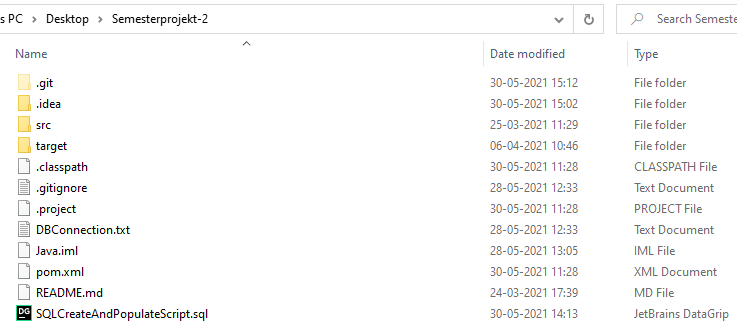
\includegraphics{images/MainFolder.PNG}
    \caption{Hoved mappen}
    \label{fig:my_label}
\end{figure}

\begin{figure}[H]
    \centering
    
\includegraphics{images/src.PNG}
    \caption{src mappen}
    \label{fig:my_label}
\end{figure}

\begin{figure}[H]
    \centering
    
\includegraphics{images/main.PNG}
    \caption{main mappen}
    \label{fig:my_label}
\end{figure}

\begin{figure}[H]
    \centering
    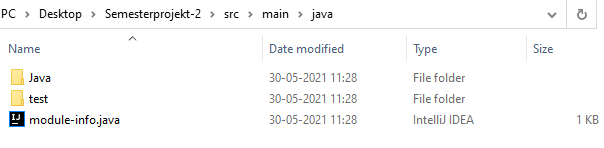
\includegraphics{images/javasmol.PNG}
    \caption{java mappen}
    \label{fig:my_label}
\end{figure}

\begin{figure}[H]
    \centering
    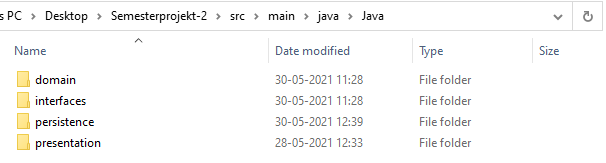
\includegraphics{images/javaBig.PNG}
    \caption{Java mappen}
    \label{fig:my_label}
\end{figure}

\begin{figure}[H]
    \centering
    
\includegraphics{images/presentation.PNG}
    \caption{Presentation mappen}
    \label{fig:my_label}
\end{figure}

\begin{figure}[H]
    \centering
    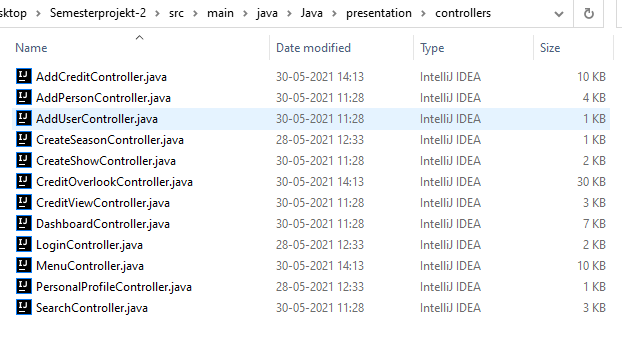
\includegraphics{images/controllers.PNG}
    \caption{Controllers mappen}
    \label{fig:my_label}
\end{figure}

\begin{figure}[H]
    \centering
    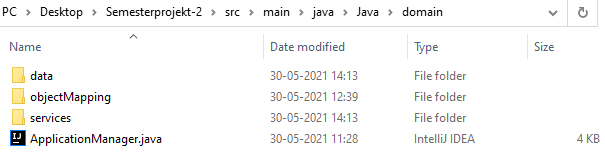
\includegraphics{images/domain.PNG}
    \caption{Domain mappen}
    \label{fig:my_label}
\end{figure}

\begin{figure}[H]
    \centering
    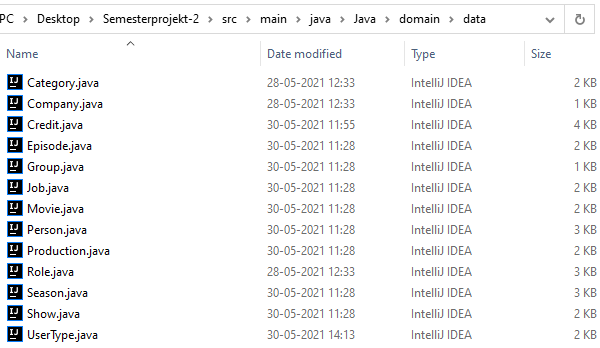
\includegraphics{images/domainData.PNG}
    \caption{Domain Data mappen}
    \label{fig:my_label}
\end{figure}

\begin{figure}
    \centering
    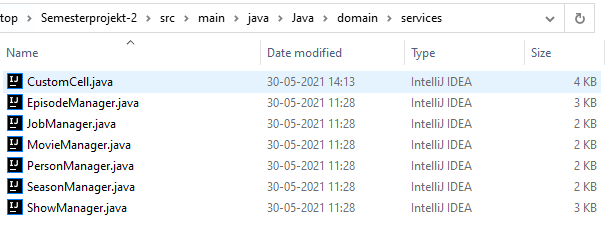
\includegraphics{images/services.PNG}
    \caption{Domain services mappen}
    \label{fig:my_label}
\end{figure}

\begin{figure}[H]
    \centering
    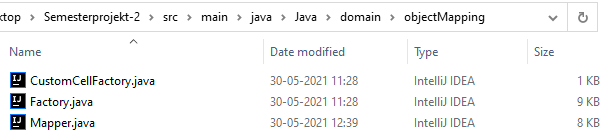
\includegraphics{images/ObjectMapping.PNG}
    \caption{ObjectMapping mappen}
    \label{fig:my_label}
\end{figure}

\begin{figure}[H]
    \centering
    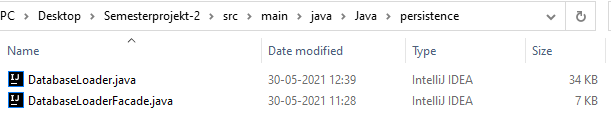
\includegraphics{images/persistence.PNG}
    \caption{Persistence Mappen}
    \label{fig:my_label}
\end{figure}

\begin{figure}[H]
    \centering
    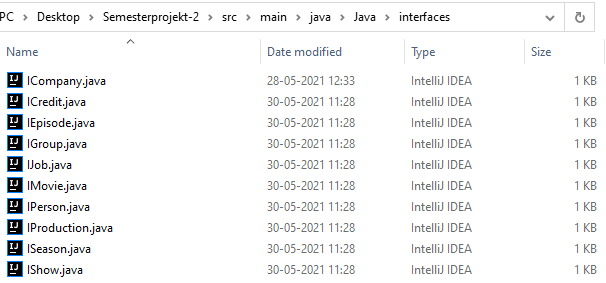
\includegraphics{images/interfaces.PNG}
    \caption{Interface mappen}
    \label{fig:my_label}
\end{figure}
\section{Brugervejledning}

Når programmet startes via intelliJ mødes du af denne skærm:

\begin{figure}[H]
    \centering
    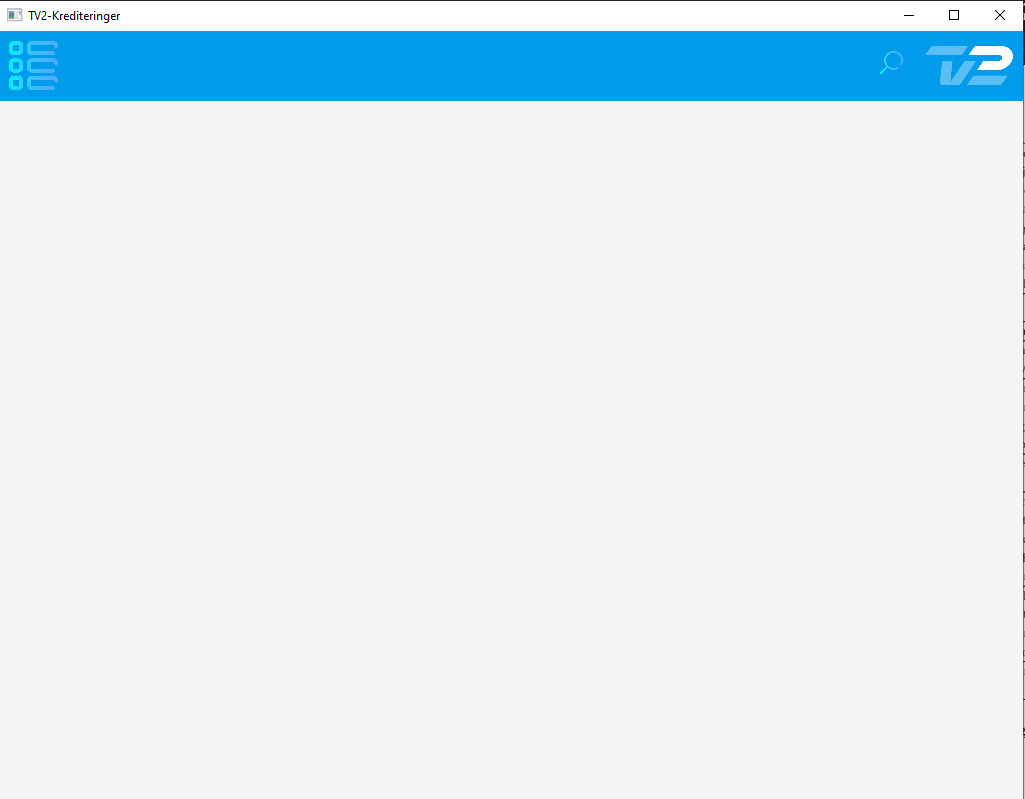
\includegraphics[scale = 0.5]{images/Home.PNG}
    \caption{Startskærm}
    \label{fig:my_label}
\end{figure}

Som standard er du ikke logget ind, og kan derfor kun foretage en søgning. For at foretage en søgning, skal du klikke til venstre for søgeknappen:

\begin{figure}[H]
    \centering
    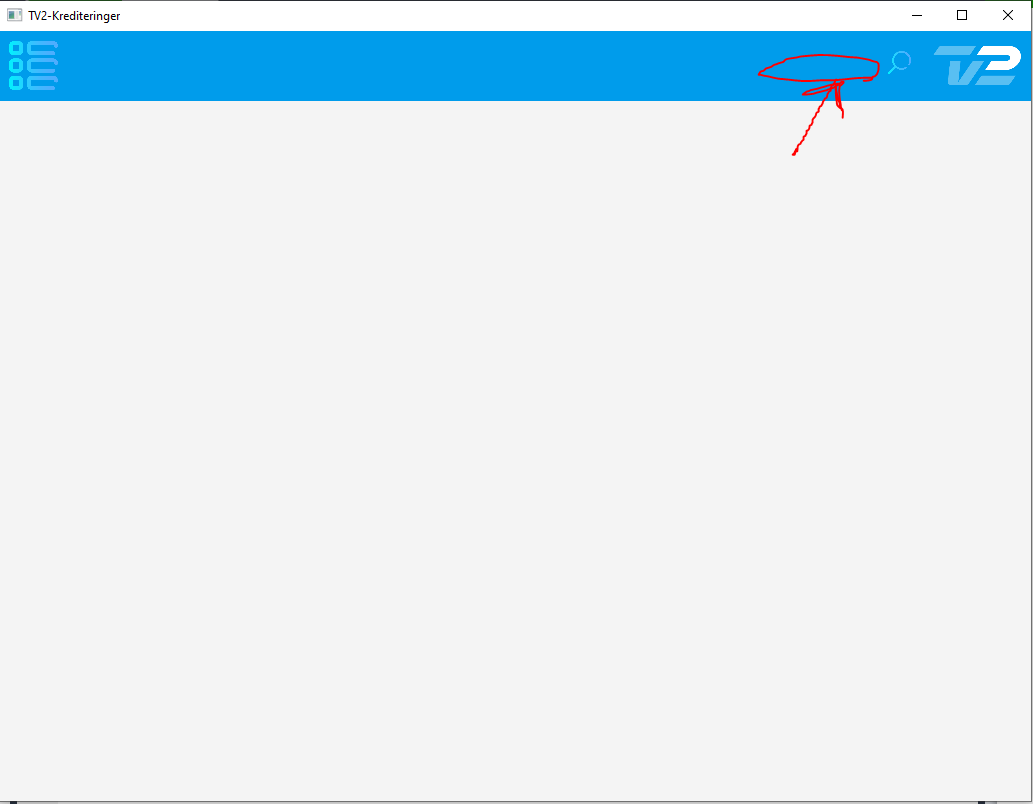
\includegraphics[scale = 0.5]{images/StartSearch.PNG}
    \caption{Start søgning}
    \label{fig:my_label}
\end{figure}

Her kan du indtaste noget tekst som du vil søge efter, og herefter trykke på forstørrelsesglasset, som vil hente alle krediteringer der svarer til teksten, og vise dig en liste.

Ønsker du at logge ind for at få muligheden for at ændre i krediteringer skal du trykke på menuen oppe til venste:

\begin{figure}[H]
    \centering
    
\includegraphics{images/OpenMenu.PNG}
    \caption{Åben menu}
    \label{fig:my_label}
\end{figure}

Her vælger du så Login:

\begin{figure}[H]
    \centering
    
\includegraphics{images/login.PNG}
    \caption{Start Login}
    \label{fig:my_label}
\end{figure}

Og du bliver så mødt af denne skærm:

\begin{figure}[H]
    \centering
    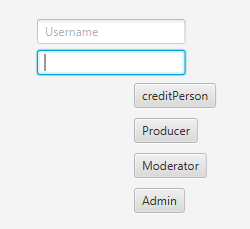
\includegraphics{images/UserTypes.PNG}
    \caption{Login skærmen}
    \label{fig:my_label}
\end{figure}

Adgangskontrollen er endnu ikke implementeret, så har anbefales at du blot vælger Admin, og så bliver du logget ind med administrator rettigheder. Du kommer nu tilbage til startskærmen, men hvis du trykke på menuen igen bliver du mødt af denne menu.

\begin{figure}[H]
    \centering
    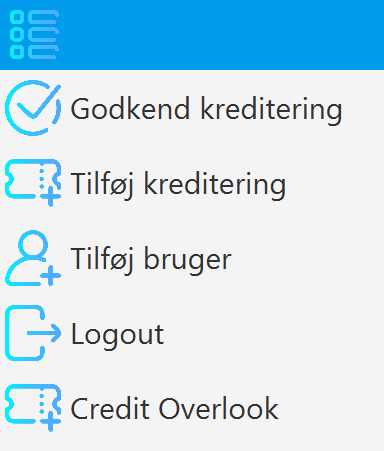
\includegraphics[scale = 0.8]{images/AdminMenu.PNG}
    \caption{Administrator menuen}
    \label{fig:my_label}
\end{figure}

Her har du adgang til alle features tilføjet i programmet. Den med avancerede er Credit Overlook, så hvis du trypper på den bliver du mødt af denne skærm:

\begin{figure}[H]
    \centering
    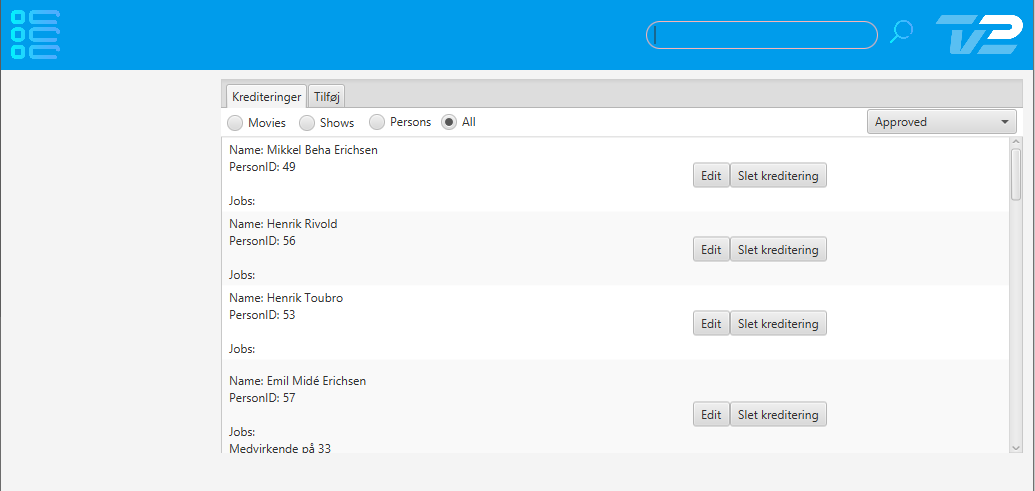
\includegraphics[scale = 0.65]{images/CreditOverlook.PNG}
    \caption{Credit overlook skærmen}
    \label{fig:my_label}
\end{figure}

Her har du nu et hav a muligheder. Øverst kan du vælge mellem "krediteringer" som viser dig alle krediteringer i systemet, som du kan sortere efter type. Eller du kan vælge tilføj, hvor du kan tilføje nye krediteringer. I toppen helt til højre kan du vælge at få vist krediteringer der er godkendt, eller venter på at blive godkendt. Da du er Admin, vil du også kunne godkende de krediteringer der ikke er godkendt. Nede ved krediteringerne Kan du vælge at trykke edit, hvor du vil kunne redigere en kreditering, eller trykke slet, som vil slette krediteringen fra databasen.
\section{Samarbejdsaftale}
\label{Gruppekontrakt}
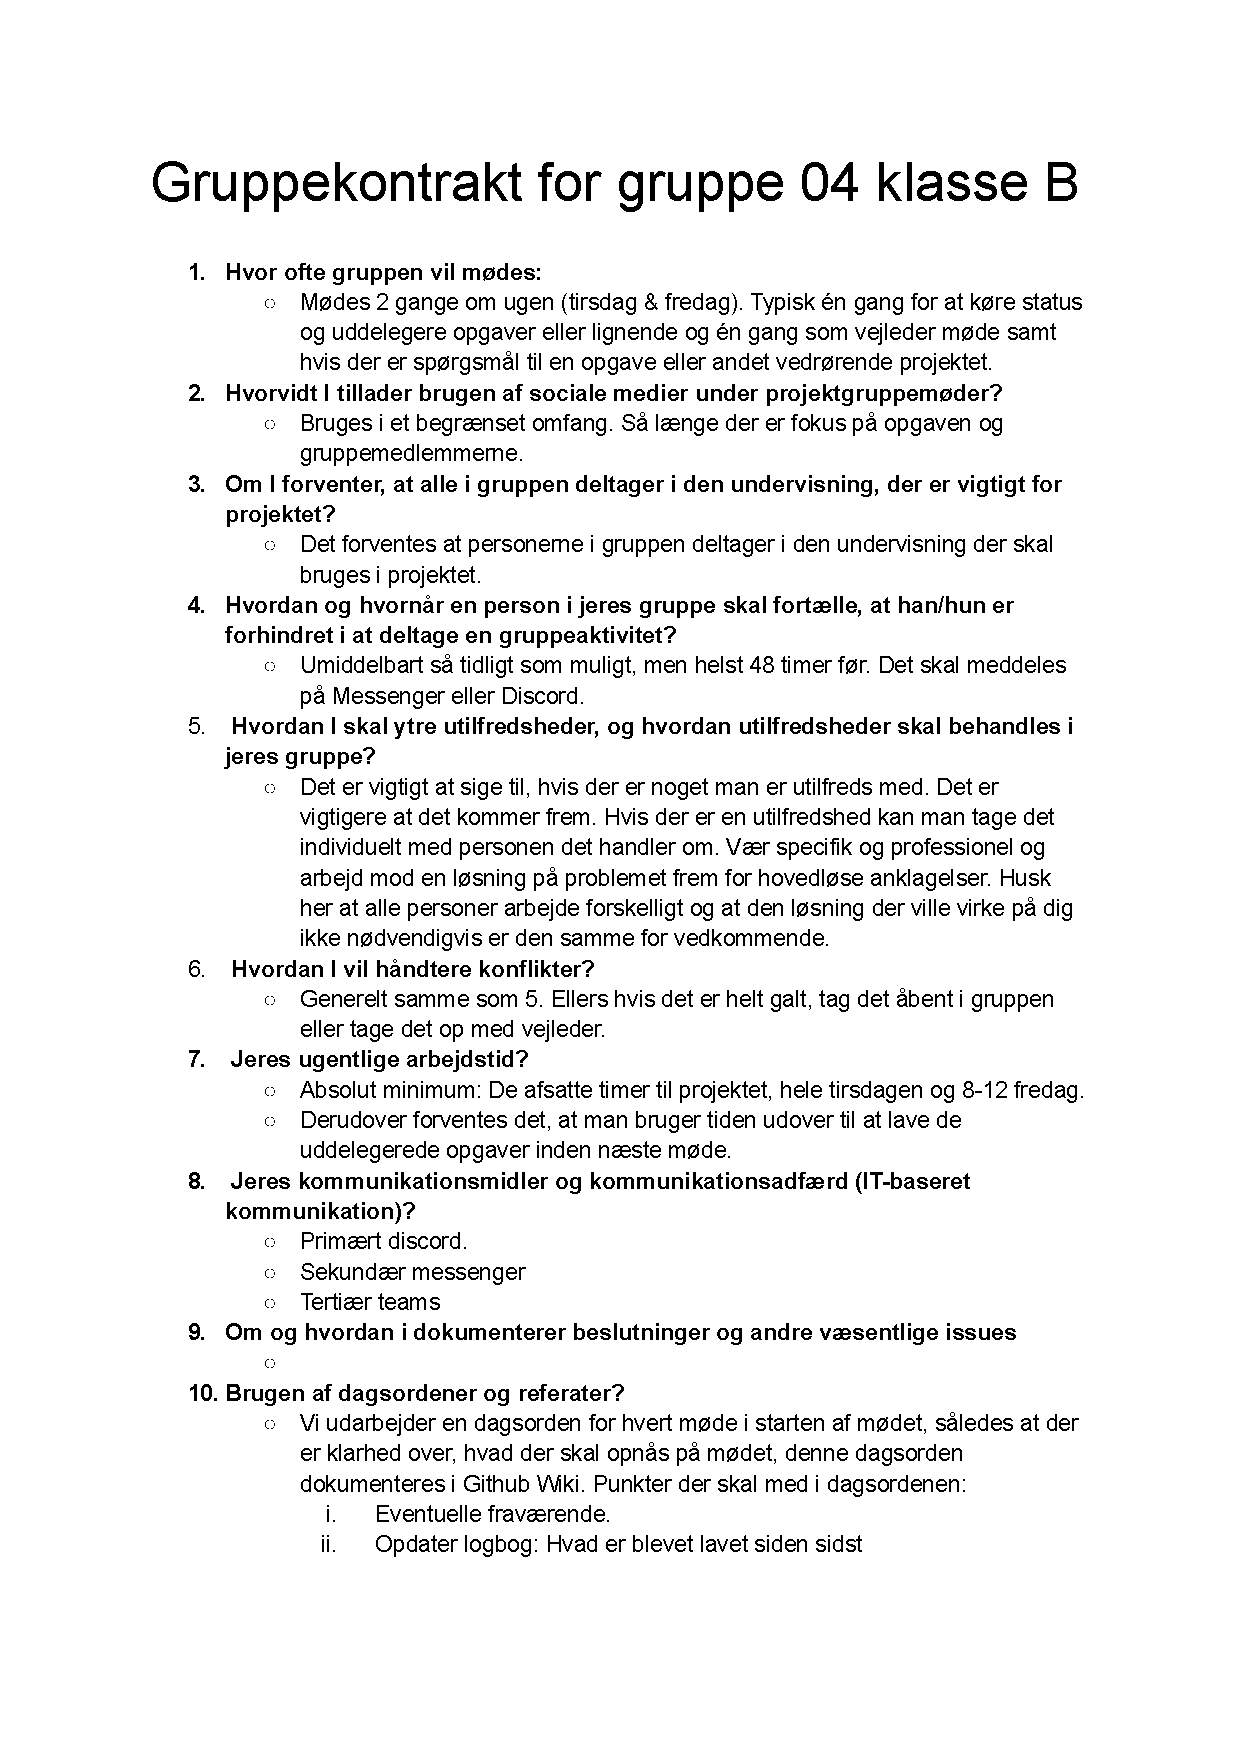
\includepdf[pagecommand={\thispagestyle{plain}}, page=-]{Bilag/Gruppekontrakt.pdf}
\section{Vejlederaftale}
Et afsnit omkring vejlederaftale findes i gruppekontrakten i bilag \ref{Gruppekontrakt}
\section{Projektlog}
Gruppeloggen kan findes på: \href{https://github.com/hannehue/Semesterprojekt-2/wiki/Gruppelog}{https://github.com/hannehue/Semesterprojekt-2/wiki/Gruppelog}
\clearpage
\section{Udfyldt rapportkontrolskema}


\begin{longtable}{|p{30mm}|p{90mm}|p{25mm}|}
\hline
\textbf{Kapitel}    & \textbf{krav}     & \textbf{Opfyldt +/-} \\ \hline

\textbf{Forside}    & Projekttitel, uddannelsesinstitution, fakultet, institut, uddannelse, semester, kursuskode, projektperiode, vejleder, projektgruppe og projektdeltagere (fornavn, efternavn, sdu-email). Må gerne have illustrationer.
                                &           \\ \hline
                                        
\textbf{Titleblad}  & Samme oplysninger som på forsiden, samt afleveringsdato og projektdeltagernes underskrifter (Projektdeltagernes aktive deltagelse i projektforløbet anerkendes gensidigt ved projektdeltagernes underskrifter). Må ikke have illustrationer.
                                &           \\ \hline
                                        
\textbf{Resumé}     & \begin{itemize}
                        \item En kort introduktion til projektet - hvad blev der arbejdet med og hvorfor.
                        \item Problemformuleringen og vigtige afgrænsninger.
                        \item Metode - hvordan angreb I problemet og hvordan realiserede I løsningen (hvem, hvad, hvornår og hvorfor)
                        \item Hovedresultater og konklusioner  – hvad kom der ud af arbejdet.
                    \end{itemize}
                        (max 1 side)
                                &           \\ \hline

\textbf{Forord}     & Hensigten med rapporten, målgruppe, forhistorie, anerkendelser.
                                &           \\ \hline

\textbf{Indholdsfor-tegnelse}    & Samlet indholdsfortegnelse for hele projektrapporten. 
Højst to eller tre niveauer i indholdsfortegnelse (der kan evt. være flere i selve rapporten). Afsnit på niveau 1 og 2 skal være nummererede.
                                &           \\ \hline

\textbf{Læsevejledning}     & Vejledning i hvordan rapporten kan læses, eksempelvis i form af hvilken rækkefølge afsnittene kan læses i, og hvordan sammenhængen er mellem de forskellige dele af rapporten, herunder mellem hovedrapport og bilag. Rapportens målgruppe.
                                &           \\ \hline

\textbf{Redaktionelt}   & Skriveprocessen og ansvarsområder i skriveprocessen.

Ansvarsområder kan fx beskrives på fx følgende form:

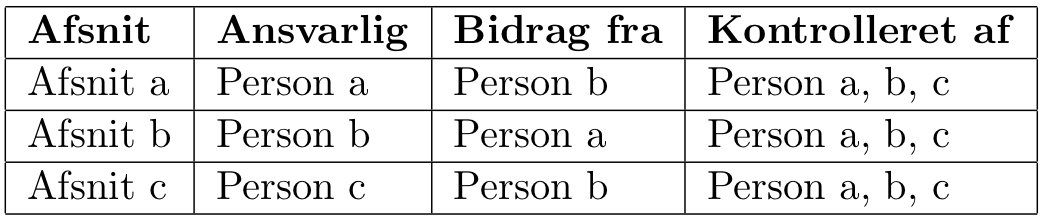
\includegraphics[scale=0.49]{images/kontolskema_bilag_F.png}

                                &           \\ \hline
                                
\textbf{Indledning}     & Projektets rammer og baggrunden for projektet.
Resume af udleverede case.
Problemformulering og afgrænsninger. 
Formål og mål med projektet.
Problemformulering og afgrænsninger. 
\textit{(indledningen må gerne includere materiale direkte fra inceptionsdokumentet, det skal blot have en tydelig reference)}
                                &           \\ \hline
                                
\textbf{Faglig vidensgrundlag}  & Begrebsdefinitioner, teori og  fagligt vidensgrundlag.
                                &           \\ \hline
                                
\textbf{Metode og planlægning} & \textbf{Metode:} 
Benyttede metoder i projekt (hele projektet).
Kombination af UP og Scrum. Fordele og ulemper
                                &           \\ \hline
                                
                            & \textbf{Planlægning:} 
Plan for elaborationsfasen og de enkelte iterationer. Prioritering af krav i planlægningen.
Det faktiske udviklingsarbejde. Faserne, iterationerne og det faktiske  arbejde i dem?
Scrum: backlogs, roller, begivenheder, scrum-buts.
                                &           \\ \hline

\textbf{Hovedtekst}
(skal indeholde resultater både fra iteration 1 og fra iteration 2)
    & \textbf{Overordnede krav:}
    Opdateret resume af overordnede krav fra inceptionsdokument inklusive overordnet brugsmønsterdiagram og oversigt over supplerende krav.
                                    &           \\ \hline
    & \textbf{Detaljerede krav:}
    Detaljeret brugsmønsterdiagram (hvis relevant).
    Detaljerede brugsmønsterbeskrivelser.
    Detaljerede beskrivelser af supplerende krav, fx organiseret efter FURPS+.
                                        &           \\ \hline
    & \textbf{Analyse:} 
    Overvejelser, beslutninger og resultater vedr. analysemodellen, inklusive både den statiske og den dynamiske side af analysemodel. 
                                        &           \\ \hline
    & \textbf{Design:}
    Overvejelser, beslutninger og resultater vedr. Softwarearkitektur og detaljeret design, herunder design af persistens. 
                                        &           \\ \hline
    & \textbf{Databasedesign:}
    Overvejelser, beslutninger og resultater vedr. tabeldesign og SQL-forespørgsler.
                                        &           \\ \hline
    & \textbf{Implementering:}
    Overvejelser, beslutninger og resultater vedr.  konvertering fra design til kode illustreret gennem udvalgte centrale eksempler, samt andre vigtige implementeringsbeslutninger. 
    Implementering af database.
                                        &           \\ \hline
    & \textbf{Test:}
    udførte test samt resultatet af dem.
                                        &           \\ \hline

\textbf{Diskussion} & Hvad er der opnået og hvad er der ikke opnået i projektet i forhold til det forventede som beskrevet i indledningen. 
Hvad er styrkerne og svaghederne ved resultaterne.
Kunne I have opnået bedre resultater?
                                        &           \\ \hline

\textbf{Konklusion} & Opsummering af resultaterne og diskussionen af dem. Svar på problemformuleringen. 
                                        &           \\ \hline

\textbf{Perspektivering}   & Er den fundne løsning brugbar i anden sammenhæng?
Hvad bidrager løsningen og den opnåede viden til. 
Fremtidigt arbejde (næste skridt i projektet, hvis I havde mere tid).
                                        &           \\ \hline

\textbf{Procesevaluering}   & Processen og gruppens refleksion over processen: Læringsprocessen, teamroller, samarbejdet internt i gruppen og med vejleder, projektarbejdsformen, arbejdsformer, metoder, skriveprocessen, den tidsmæssige styring af projektet,ledelse af projektet, arbejdsfordeling i projektet m.m. 
Hvordan ville I gribe arbejdet an, hvis I skulle starte forfra?
                                        &           \\ \hline

\textbf{Referenceliste}   & Litteratur angivet på en anerkendt form. 
(Alle former for litteratur som bøger, artikler og hjemmesider)
Kildehenvisninger i teksten. Materiale som gruppen ikke selv har fremstillet i dette projekt skal være angivet med kilde! 
Alle kildehenvisninger i teksten skal være anført på samme måde. Kildeangivelser på figurer, grafer etc. som projektgruppen ikke selv har frembragt. 
                                        &           \\ \hline

\textbf{Bilag}   &
\makecell[l]{
A. Oversigt over kildekode \\
B. Brugervejledning \\
C. Samarbejdsaftale \\
D. Vejlederaftale \\
E. Projektlog \\
F. Udfyldt rapportkontrolskema \\
G. Inceptionsdokument \\
I.  (Andre Bilag) \\
}
                                        &           \\ \hline

\end{longtable}

\begin{longtable}{|p{30mm}|p{90mm}|p{25mm}|}
\hline
\multicolumn{3}{|c|}{\textbf{Rapporttekniske elementer}} \\ \hline

\textbf{Layout} & Er der anvendt samme layout i alle kapitler. 
Er layout overskueligt/harmonisk.
                                        &           \\ \hline

\textbf{Sprog} & Formidler rapporten projektet faglig og sagligt.
Er sproget  neutralt, aktivt, upersonligt, konkret, præcist, kortfattet og korrekt.
(Procesevalueringen må benytte personligt sprog)
                                        &           \\ \hline

\textbf{Sidenummerer-ing} & Er der korrekt og konsistent sidenummerering i rapporten. 
                                        &           \\ \hline

\textbf{Figurer/dia-grammer} & Er alle figurer konsekvent nummererede.
Er der figurtitel og figurtekst til alle figurer.
Er figurtitler og figurtekster dækkende og afklarende.
Er figurerne tydelige og læsbare.
Er figurerne informationsgivende og i den rette sammenhæng.
                                        &           \\ \hline

\textbf{Tabeller} & Er alle tabeller konsekvent nummererede.
Er der en forklarende tabeltekst til alle tabeller.
Er alle søjler og rækker forsynet med parametre.
Er der enheder på alle relevante rækker og søjler.
                                        &           \\ \hline

\textbf{Sporbarhed af begreber} & Er der en konsekvent brug af samme betegnelse for et givet begreb igennem rapporten. 
                                        &           \\ \hline



\end{longtable}


\section{Inceptionsdokument}
%\includepdf[pagecommand={\thispagestyle{plain}}, page=-]{Bilag/G_inceptionsdokument_1.pdf}


\end{document}
